\documentclass[landscape]{report}
\usepackage[legalpaper,bindingoffset=0.2in,%
            left=1cm,right=1cm,top=1in,bottom=1in,%
            footskip=.25in]{geometry}
\usepackage{tikz}
\usetikzlibrary{arrows.meta}

\begin{document}
\thispagestyle{empty}

\begin{figure}
\begin{center}

% \begin{tikzpicture}[every node/.style={draw=blue,thick,circle,inner sep=0pt}]
%   \draw[help lines,step=.5cm] (-5,-5) grid (5,5);
%   \node[minimum size=8cm] (4,2)  {};
%   \node  (a1) at (4,2) { # };
% \end{tikzpicture} 


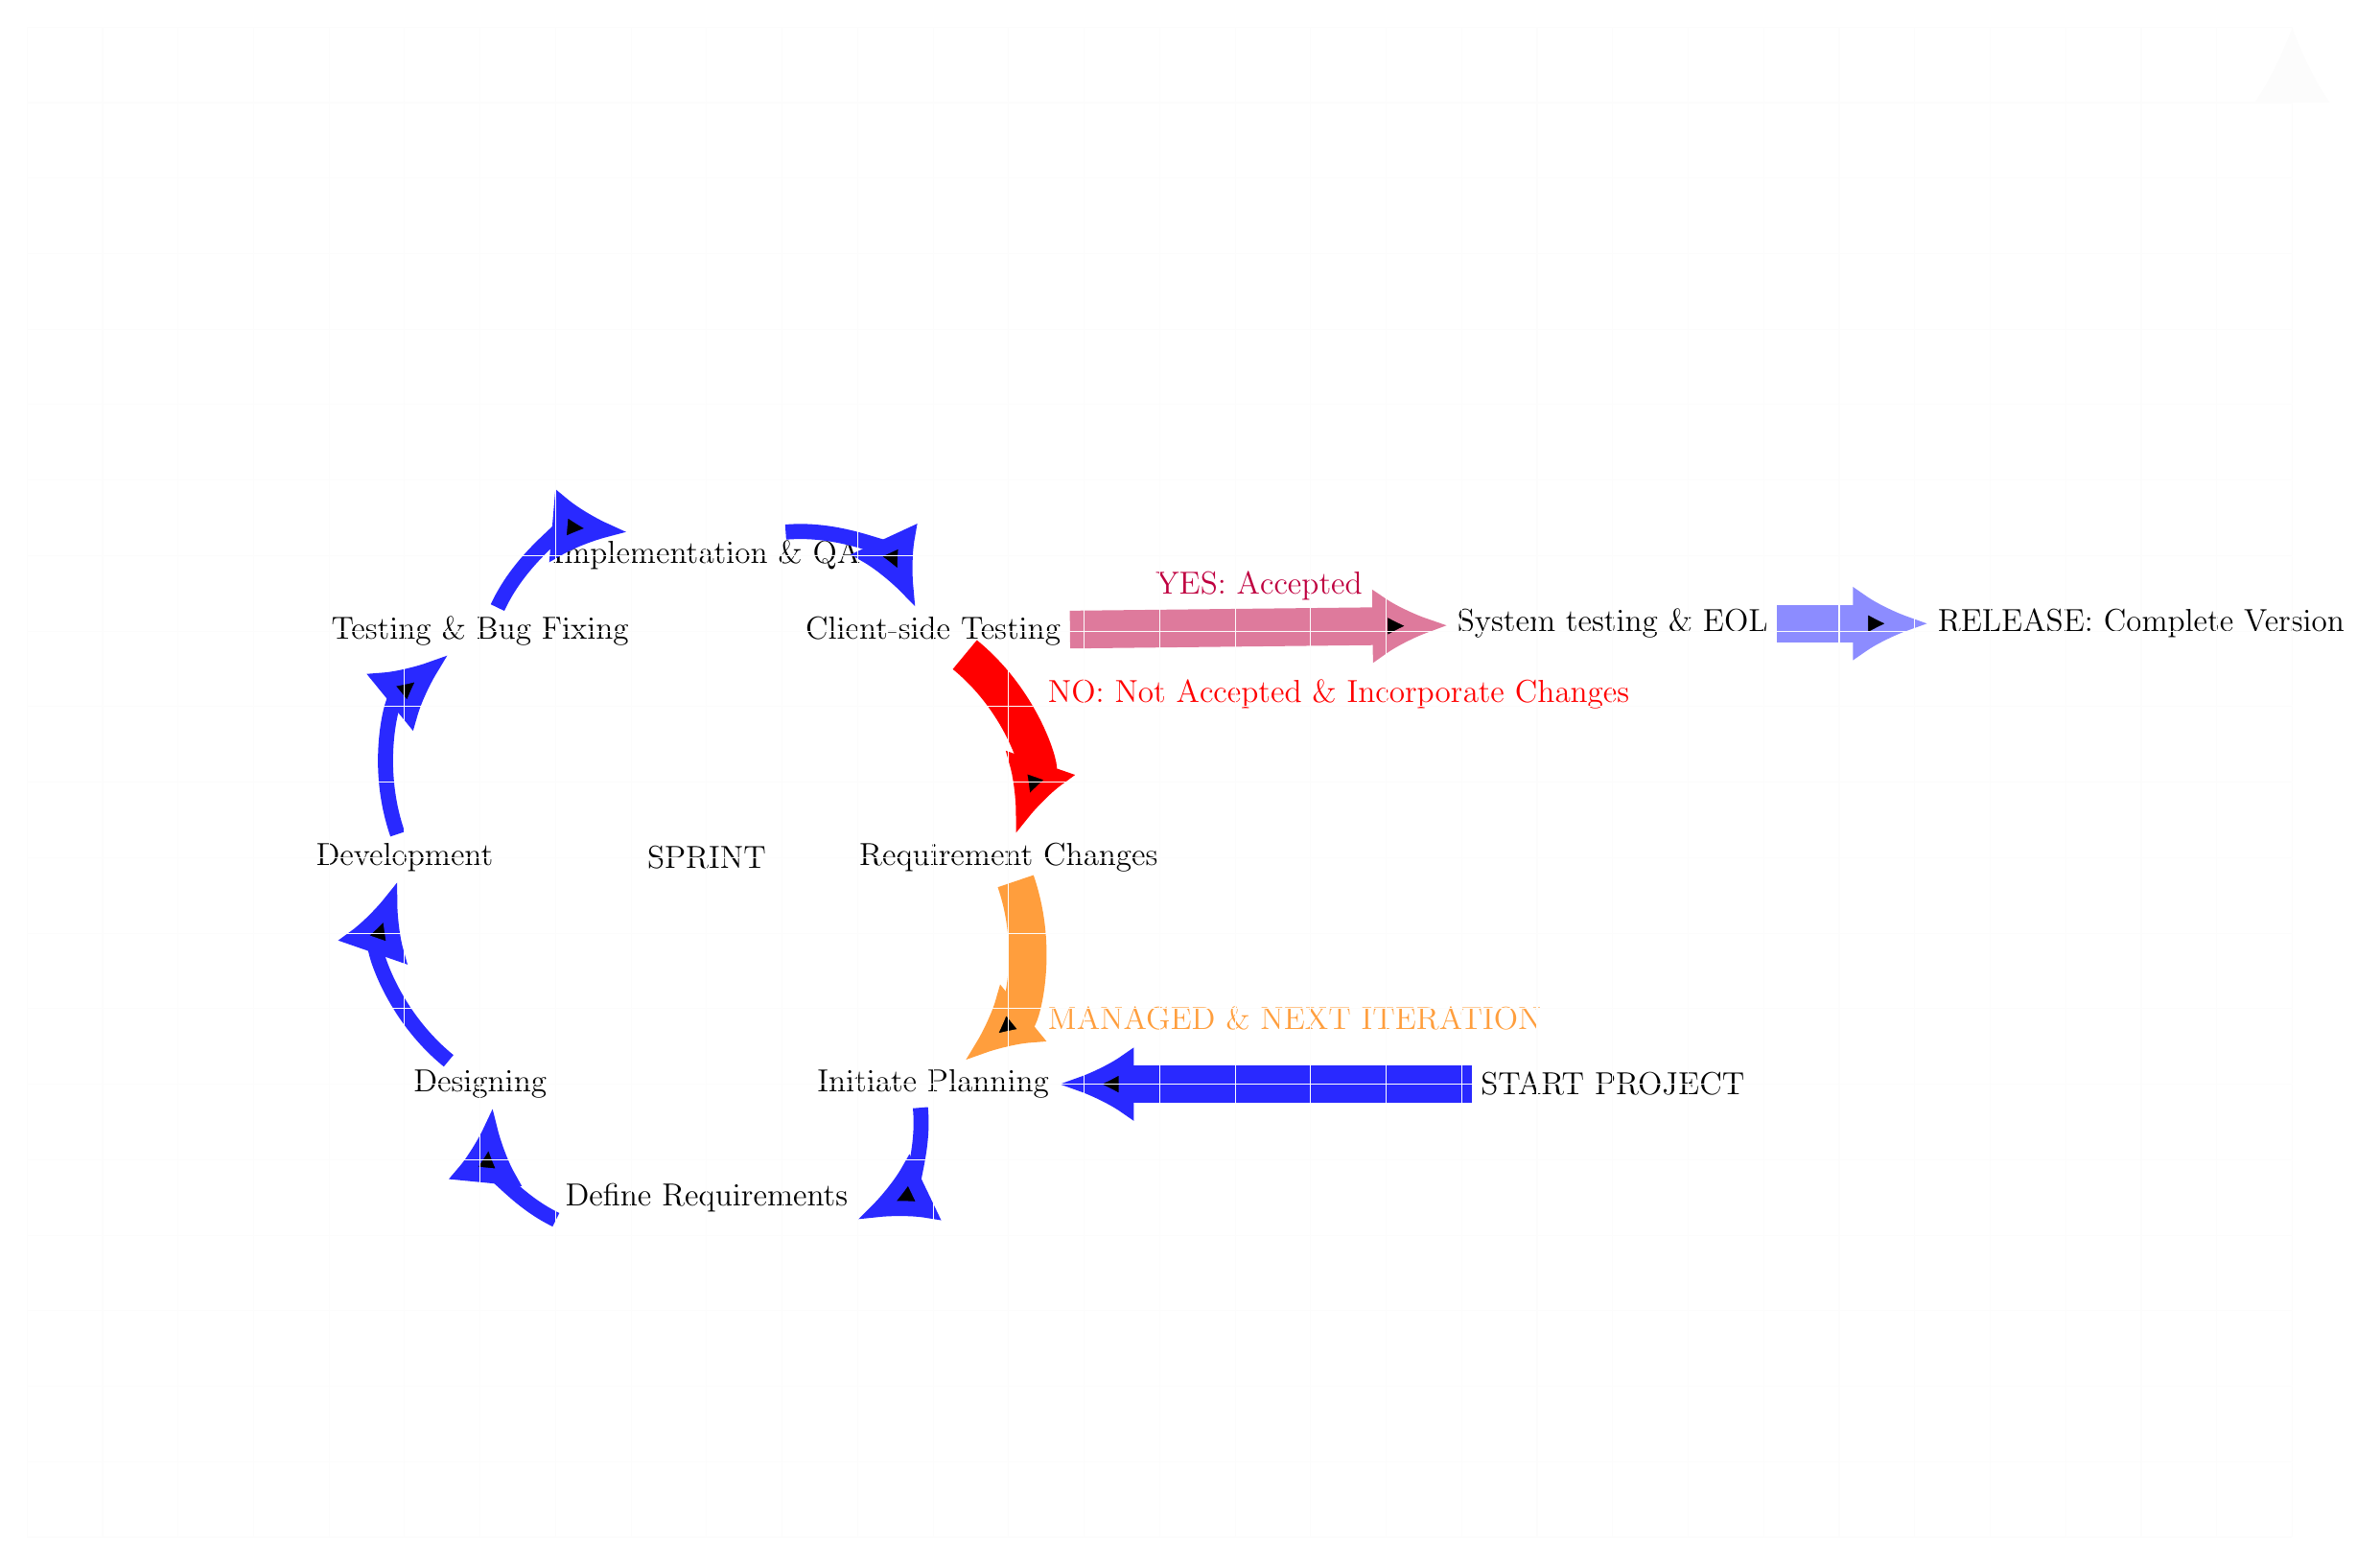
\begin{tikzpicture}[node distance=1.3cm,bend angle=35,auto,>={LaTeX[width=10mm,length=10mm]},->]
\tikzstyle{every node}=[font=\large]
\node (s11) at (4,4) { SPRINT };

\node  (f1) at (16,7.1) { System testing \& EOL};
\node  (f2) at (23,7.1) { RELEASE: Complete Version};
\node  (start) at (16,1) { START PROJECT };

\node  (start1) at (7,1) { Initiate Planning };
\node  (s1) at (4,-.5) { Define Requirements };
\node  (s2) at (1,1) { Designing };
\node  (s3) at (0,4) { Development };
\node  (s4) at (1,7) { Testing \& Bug Fixing };
\node  (s5) at (4,8) { Implementation \& QA};
\node  (s6) at (7,7) { Client-side Testing };
\node  (s7) at (8,4) { Requirement Changes};

\path[line width=5mm,draw=blue!84] (start) edge node{} (start1);

\path[->,line width=2mm,draw=blue!84] (s1) edge [bend left] (s2);
\path[->,line width=2mm,draw=blue!84] (s2) edge [bend left] (s3);
\path[->,line width=2mm,draw=blue!84] (s3) edge [bend left] (s4);
\path[->,line width=2mm,draw=blue!84] (s4) edge [bend left] (s5);
\path[->,line width=2mm,draw=blue!84] (s5) edge [bend left] (s6);
\path[->,line width=2mm,draw=blue!84] (start1) edge [bend left] (s1);

\path[->,line width=5mm,draw=red] (s6) edge [bend left] node {\color{red}{NO: Not Accepted \& Incorporate Changes} }(s7);
\path[->,line width=5mm,draw=orange!76] (s7) edge [bend left] node {\color{orange!76}MANAGED \& NEXT ITERATION}(start1);

\path[line width=5mm,draw=purple!52] (s6) edge node {\color{purple}{YES: Accepted}}(f1);
\path[line width=5mm,draw=blue!45] (f1) edge node{} (f2);


%\draw[blue!2, thin] (-15,-15) grid (15,15);
\draw[black!1,thin,step=1cm] (-5,-5) grid (25,15);

\end{tikzpicture}
\end{center}
% \caption{First (faulty) version of a timed automaton for processing
%   emergency messages} 
% \label{fig:ta:emergency1}
\end{figure}

\end{document}


% convert           \
%    -verbose       \
%    -density 1000   \
%    -trim          \
%     Agile-DevelopmentModel.pdf      \
%    -quality 1000   \
%    -flatten       \
%    -sharpen 0x1.0 \
%     Agile-DevelopmentModel.png
